\documentclass{standalone}

\usepackage{graphicx}

\usepackage{tikz}
\usetikzlibrary{calc}
\usetikzlibrary{positioning}
\tikzset{
    between/.style args={#1 and #2}{
    	at = ($(#1)!0.5!(#2)$)
    }
}

\begin{document}

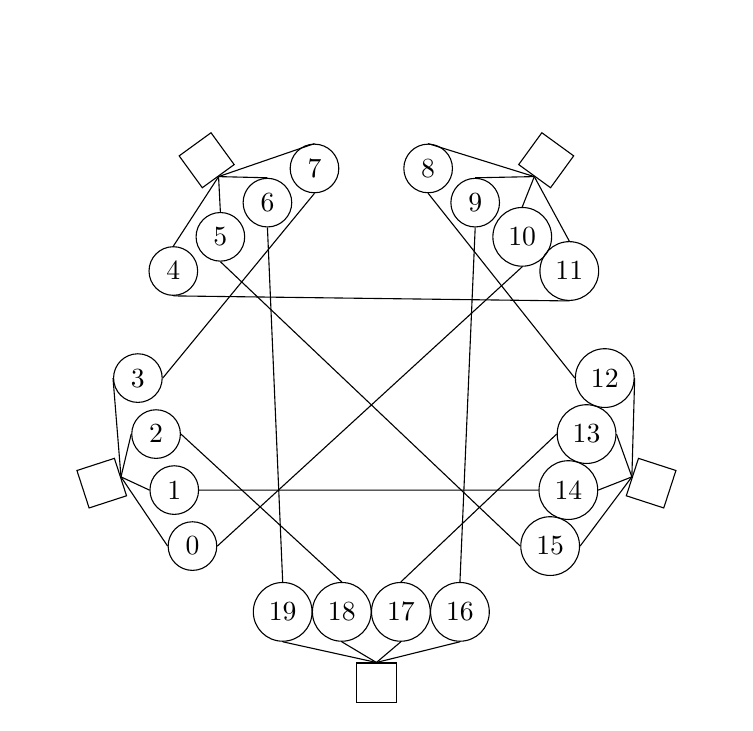
\begin{tikzpicture}[
        % every node/.style={node distance=6mm and 1mm},
        server/.style={circle, draw=black},
        switch/.style={rectangle, draw=black, minimum size=.5cm},
    ]

    \def \sidelen {4};
    \def \osidemargin {.8};
    \def \podservers {4};
    \def \intangle {108};

    \pgfmathsetmacro \adj {{cos(180 - \intangle) * \sidelen}};
    \pgfmathsetmacro \opp {{sin(180 - \intangle) * \sidelen}};
    \pgfmathsetmacro \adjb {{sin(36) * \sidelen}};
    \pgfmathsetmacro \oppb {{cos(36) * \sidelen}};

    \pgfmathsetmacro \osidelen{2 * cos(54) * sqrt(\osidemargin^2 + \osidemargin^2) + \sidelen};

    \pgfmathsetmacro \oadj {{cos(180 - \intangle) * \osidelen}};
    \pgfmathsetmacro \oopp {{sin(180 - \intangle) * \osidelen}};
    \pgfmathsetmacro \oadjb {{sin(36) * \osidelen}};
    \pgfmathsetmacro \ooppb {{cos(36) * \osidelen}};

    % Corner points of the inner pentagon
    \pgfmathsetmacro \xshft {-.2}
    \pgfmathsetmacro \yshft {.1}

    \node[] (C1) at (0 + \xshft, 0 + \yshft) {};
    \node[] (C2) at (-\adj + \xshft, \opp + \yshft) {};
    \node[] (C3) at (-\adj + \oppb + \xshft, \opp + \adjb + \yshft) {};
    \node[] (C4) at (\sidelen + \adj + \xshft, \opp + \yshft) {};
    \node[] (C5) at (\sidelen + \xshft, 0 + \yshft) {};

    % Corner points of the outer pentagon
    \node[] (CO1) at (-\osidemargin,- \osidemargin) {};
    \node[] (CO2) at (-\osidemargin - \oadj, - \osidemargin + \oopp) {};
    \node[] (CO3) at (-\osidemargin - \oadj + \ooppb, \oopp + \oadjb -\osidemargin) {};
    \node[] (CO4) at (-\osidemargin + \osidelen + \oadj, \oopp - \osidemargin) {};
    \node[] (CO5) at (-\osidemargin + \osidelen, -\osidemargin) {};

    % \draw[-] (CO1) -- (CO2);
    % \draw[-] (CO2) -- (CO3);
    % \draw[-] (CO3) -- (CO4);
    % \draw[-] (CO4) -- (CO5);
    % \draw[-] (CO5) -- (CO1);

    \path[-] (CO1) -- (CO2)
    node[switch, pos=0.5, rotate = 288] (SW1)   {};
    \path[-] (CO2) -- (CO3)
    node[switch, pos=0.5, rotate = 216] (SW2)   {};
    \path[-] (CO3) -- (CO4)
    node[switch, pos=0.5, rotate=144] (SW3)   {};
    \path[-] (CO4) -- (CO5)
    node[switch, pos=0.5, rotate=72] (SW4)   {};
    \path[-] (CO5) -- (CO1)
    node[switch, pos=0.5, rotate=0] (SW5)   {};

    \path (C1) -- (C2)
    node[server, pos=0.2] (S1)   {0}
    node[server, pos=0.4] (S2)   {1}
    node[server, pos=0.6] (S3)   {2}
    node[server, pos=0.8] (S4)   {3};

    \path (C2) -- (C3)
    node[server, pos=0.2] (S5)   {4}
    node[server, pos=0.4] (S6)   {5}
    node[server, pos=0.6] (S7)   {6}
    node[server, pos=0.8] (S8)   {7};

    \path (C3) -- (C4)
    node[server, pos=0.2] (S9)   {8}
    node[server, pos=0.4] (S10)  {9}
    node[server, pos=0.6] (S11)  {10}
    node[server, pos=0.8] (S12)  {11};

    \path (C4) -- (C5)
    node[server, pos=0.2] (S13)  {12}
    node[server, pos=0.4] (S14)  {13}
    node[server, pos=0.6] (S15)  {14}
    node[server, pos=0.8] (S16)  {15};

    \path (C5) -- (C1)
    node[server, pos=0.2] (S17)  {16}
    node[server, pos=0.4] (S18)  {17}
    node[server, pos=0.6] (S19)  {18}
    node[server, pos=0.8] (S20)  {19};

    \draw[-] (S9.south)  -- (S13.west);
    \draw[-] (S10.south)  -- (S17.north);
    \draw[-] (S11.south)  -- (S1.east);
    \draw[-] (S12.south)  -- (S5.south);

    \draw[-] (S14.west)  -- (S18.north);
    \draw[-] (S15.west)  -- (S2.east);
    \draw[-] (S16.west)  -- (S6.south);

    \draw[-] (S19.north)  -- (S3.east);
    \draw[-] (S20.north)  -- (S7.south);

    \draw[-] (S4.east)  -- (S8.south);

    \draw[-] (S1.west)  -- (SW1.north);
    \draw[-] (S2.west)  -- (SW1.north);
    \draw[-] (S3.west)  -- (SW1.north);
    \draw[-] (S4.west)  -- (SW1.north);

    \draw[-] (S5.north)  -- (SW2.north);
    \draw[-] (S6.north)  -- (SW2.north);
    \draw[-] (S7.north)  -- (SW2.north);
    \draw[-] (S8.north)  -- (SW2.north);

    \draw[-] (S9.north)  -- (SW3.north);
    \draw[-] (S10.north)  -- (SW3.north);
    \draw[-] (S11.north)  -- (SW3.north);
    \draw[-] (S12.north)  -- (SW3.north);

    \draw[-] (S13.east)  -- (SW4.north);
    \draw[-] (S14.east)  -- (SW4.north);
    \draw[-] (S15.east)  -- (SW4.north);
    \draw[-] (S16.east)  -- (SW4.north);

    \draw[-] (S17.south)  -- (SW5.north);
    \draw[-] (S18.south)  -- (SW5.north);
    \draw[-] (S19.south)  -- (SW5.north);
    \draw[-] (S20.south)  -- (SW5.north);
\end{tikzpicture}

\end{document}